%% LyX 1.3 created this file.  For more info, see http://www.lyx.org/.
%% Do not edit unless you really know what you are doing.
\documentclass[english, 12pt]{article}
\usepackage{times}
%\usepackage{algorithm2e}
\usepackage{url}
\usepackage{bbm}
\usepackage[T1]{fontenc}
\usepackage[latin1]{inputenc}
\usepackage{geometry}
\geometry{verbose,letterpaper,tmargin=2cm,bmargin=2cm,lmargin=1.5cm,rmargin=1.5cm}
\usepackage{rotating}
\usepackage{color}
\usepackage{graphicx}
\usepackage{amsmath, amsthm, amssymb}
\usepackage{setspace}
\usepackage{lineno}
\usepackage{hyperref}
\usepackage{bbm}
\usepackage{makecell}
\usepackage{placeins}
\usepackage{subcaption}

%\renewcommand{\arraystretch}{1.8}

%\usepackage{xr}
%\externaldocument{SCT-supp}

%\linenumbers
%\doublespacing
\onehalfspacing
%\usepackage[authoryear]{natbib}
\usepackage{natbib} \bibpunct{(}{)}{;}{author-year}{}{,}

%Pour les rajouts
\usepackage{color}
\definecolor{trustcolor}{rgb}{0,0,1}

\usepackage{dsfont}
\usepackage[warn]{textcomp}
\usepackage{adjustbox}
\usepackage{multirow}
\usepackage{graphicx}
\graphicspath{{../figures/}}
\DeclareMathOperator*{\argmin}{\arg\!\min}

\let\tabbeg\tabular
\let\tabend\endtabular
\renewenvironment{tabular}{\begin{adjustbox}{max width=0.95\textwidth}\tabbeg}{\tabend\end{adjustbox}}

\makeatletter

%%%%%%%%%%%%%%%%%%%%%%%%%%%%%% LyX specific LaTeX commands.
%% Bold symbol macro for standard LaTeX users
%\newcommand{\boldsymbol}[1]{\mbox{\boldmath $#1$}}

%% Because html converters don't know tabularnewline
\providecommand{\tabularnewline}{\\}
\renewcommand*{\arraystretch}{1.2}

\usepackage{babel}
\makeatother


\begin{document}

\renewcommand{\thefigure}{S\arabic{figure}}
\setcounter{figure}{0}
\renewcommand{\thetable}{S\arabic{table}}
\setcounter{table}{0}
\renewcommand{\theequation}{S\arabic{equation}}
\setcounter{equation}{0}

%%%%%%%%%%%%%%%%%%%%%%%%%%%%%%%%%%%%%%%%%%%%%%%%%%%%%%%%%%%%%%%%%%%%%%%%%%%%%%%%

\subsection*{Simulations}

\begin{table}[ht]
	\centering
	\begin{tabular}{|l|c|c|c|c|c|c|c|}
		\hline
		Method & all\_40\_300 & all\_40\_3000 & all\_40\_30000 & all\_40\_300000 & both\_40 & HLA\_30\_300 & HLA\_30\_3000 \\
		\hline
		LDpred1-inf & 68.9 [68.4-69.3] & 69.3 [68.9-69.6] & 69.5 [69.2-69.7] & 69.5 [69.3-69.6] & 62.9 [61.6-64.3] & 54.4 [52.9-55.9] & 54.5 [53.7-55.5] \\
		LDpred2-inf-perchr & 70.3 [69.9-70.6] & 70.0 [69.7-70.2] & 69.9 [69.7-70.1] & 69.9 [69.7-70.0] & 74.2 [73.8-74.5] & 75.6 [74.8-76.3] & 75.7 [75.4-75.9] \\
		LDpred1-grid & 73.6 [72.0-75.4] & 70.4 [69.8-70.9] & 69.1 [68.8-69.3] & 69.2 [69.0-69.4] & 61.7 [60.4-63.1] & 54.7 [53.9-55.5] & 54.5 [53.8-55.1] \\
		LDpred2-grid-nosp-perchr & 81.7 [81.6-81.9] & 78.9 [78.7-79.0] & 70.6 [70.4-70.8] & 69.3 [69.0-69.6] & 72.8 [67.3-75.7] & 76.4 [75.7-77.0] & 76.4 [76.1-76.6] \\
		LDpred2-grid-sp-perchr & 81.7 [81.6-81.9] & 78.8 [78.7-78.9] & 70.5 [70.3-70.7] & 69.4 [69.1-69.6] & 72.8 [67.3-75.7] & 76.5 [75.8-77.1] & 76.5 [76.3-76.7] \\
		LDpred2-auto-perchr & 82.0 [81.8-82.2] & 79.3 [79.2-79.4] & 70.8 [70.6-71.0] & 69.8 [69.6-70.0] & 73.7 [73.3-74.2] & 73.1 [72.0-74.1] & 72.9 [71.6-74.0] \\
		\hline
	\end{tabular}
\end{table}


\begin{table}[ht]
	\centering
	\begin{tabular}{|l|c|c|c|c|c|}
		\hline
		Method & 10000 & 20000 & 50000 & 120000 & 300000 \\
		\hline
		LDpred1-grid & 56.1 [55.8-56.4] & 59.3 [58.9-59.8] & 66.3 [65.2-67.1] & 70.7 [69.2-71.7] & 70.4 [69.8-70.9] \\
		LDpred1-inf & 55.7 [55.4-56.0] & 57.7 [57.4-58.0] & 61.2 [60.9-61.5] & 65.0 [64.7-65.3] & 69.3 [69.0-69.7] \\
		LDpred2-auto-gwide & 55.9 [55.5-56.2] & 59.3 [58.9-59.8] & 67.5 [67.3-67.8] & 74.7 [74.6-74.9] & 79.3 [79.2-79.4] \\
		LDpred2-auto-perchr & 54.1 [53.7-54.5] & 57.3 [56.8-57.8] & 66.6 [66.3-66.9] & 74.7 [74.5-74.8] & 79.3 [79.2-79.4] \\
		LDpred2-grid-nosp-gwide & 55.7 [55.2-56.0] & 59.6 [59.3-60.0] & 67.4 [67.2-67.7] & 74.6 [74.5-74.8] & 79.1 [79.0-79.3] \\
		LDpred2-grid-nosp-perchr & 54.4 [54.0-54.8] & 58.6 [58.1-59.1] & 66.8 [66.5-67.1] & 74.2 [73.9-74.5] & 78.9 [78.7-79.0] \\
		LDpred2-grid-sp-gwide & 56.1 [55.7-56.5] & 59.6 [59.3-60.0] & 67.4 [67.2-67.7] & 74.6 [74.4-74.8] & 79.2 [79.1-79.3] \\
		LDpred2-grid-sp-perchr & 54.5 [54.2-54.9] & 58.4 [57.9-58.9] & 66.8 [66.6-67.1] & 74.2 [73.9-74.4] & 78.8 [78.7-78.9] \\
		LDpred2-inf-gwide & 55.5 [55.2-55.8] & 57.7 [57.5-58.0] & 61.4 [61.1-61.6] & 65.4 [65.1-65.6] & 69.9 [69.7-70.1] \\
		LDpred2-inf-perchr & 54.6 [54.3-55.0] & 57.2 [56.8-57.5] & 61.3 [61.0-61.5] & 65.4 [65.2-65.6] & 70.0 [69.7-70.2] \\
		\hline
	\end{tabular}
\end{table}

\FloatBarrier

%%%%%%%%%%%%%%%%%%%%%%%%%%%%%%%%%%%%%%%%%%%%%%%%%%%%%%%%%%%%%%%%%%%%%%%%%%%%%%%%

\subsection*{Real data}

\begin{table}[ht]
	\centering
	\begin{tabular}{|l|c|c|c|c|c|c|c|c|}
		\hline
		Method & Asthma & BRCA & CAD & MDD & PRCA & RA & T1D & T2D \\
		\hline
		LDpred2-grid-nosp-perchr & 58.8 [58.5-59.1] & 64.6 [64.1-65.1] & 61.5 [61.0-62.0] & 57.9 [57.5-58.2] & 68.2 [67.6-68.7] & 59.9 [59.2-60.6] & 77.0 [75.2-78.8] & 63.3 [62.9-63.7] \\
		LDpred2-grid-sp-perchr & 58.5 [58.2-58.8] & 64.6 [64.1-65.0] & 61.2 [60.8-61.7] & 58.2 [57.8-58.6] & 67.8 [67.3-68.4] & 60.0 [59.3-60.7] & 75.9 [74.0-77.7] & 63.2 [62.7-63.6] \\
		LDpred2-auto-perchr & 58.2 [57.9-58.5] & 65.6 [65.2-66.1] & 62.1 [61.6-62.6] & 58.9 [58.5-59.2] & 70.2 [69.6-70.7] & 59.7 [58.9-60.4] & 76.6 [74.7-78.5] & 63.9 [63.5-64.3] \\
		LDpred2-inf-perchr & 57.1 [56.8-57.4] & 61.9 [61.4-62.4] & 60.8 [60.4-61.3] & 58.9 [58.5-59.2] & 65.0 [64.4-65.6] & 59.6 [58.9-60.3] & 74.5 [72.6-76.3] & 61.5 [61.1-61.9] \\
		LDpred2-inf-gwide & 57.2 [56.9-57.4] & 61.6 [61.2-62.1] & 61.6 [61.1-62.1] & 59.0 [58.6-59.3] & 64.4 [63.8-65.0] & 59.3 [58.6-60.0] & 71.0 [69.1-72.8] & 61.6 [61.1-62.0] \\
		LDpred2-grid-nosp-gwide & 59.3 [59.0-59.6] & 65.5 [65.0-66.0] & 63.6 [63.2-64.1] & 59.1 [58.7-59.4] & 70.2 [69.6-70.7] & 60.3 [59.6-61.0] & 78.4 [76.7-80.2] & 64.3 [63.8-64.7] \\
		LDpred2-grid-sp-gwide & 59.4 [59.1-59.7] & 65.7 [65.3-66.2] & 63.5 [63.1-64.0] & 59.0 [58.7-59.4] & 70.2 [69.6-70.7] & 60.5 [59.8-61.3] & 78.3 [76.5-80.0] & 64.0 [63.6-64.5] \\
		LDpred2-auto-gwide & 58.4 [58.2-58.7] & 65.6 [65.2-66.1] & 61.8 [61.3-62.3] & 59.0 [58.6-59.4] & 70.1 [69.5-70.7] & 59.7 [59.0-60.4] & 77.7 [75.9-79.4] & 63.8 [63.3-64.2] \\
		LDpred1-grid & 58.6 [58.3-58.8] & 58.9 [58.4-59.4] & 60.3 [59.9-60.8] & 56.4 [56.1-56.8] & 63.5 [62.9-64.1] & 59.1 [58.4-59.8] & 57.4 [55.5-59.2] & 50.3 [49.8-50.7] \\
		LDpred1-inf & 56.9 [56.6-57.1] & 58.8 [58.3-59.3] & 59.3 [58.9-59.8] & 56.5 [56.1-56.8] & 61.6 [61.0-62.3] & 59.5 [58.8-60.2] & 57.7 [55.8-59.5] & 51.8 [51.4-52.2] \\
		\hline
	\end{tabular}
\end{table}


\begin{table}[ht]
\centering
\begin{tabular}{|l|c|c|c|c|c|c|c|c|}
	\hline
	Method & Asthma & BRCA & CAD & MDD & PRCA & RA & T1D & T2D \\
	\hline
	LDpred2-inf-gwide & 57.2 [56.9-57.4] & 61.6 [61.1-62.1] & 61.6 [61.1-62.0] & 59.0 [58.6-59.3] & 64.4 [63.8-65.0] & 59.3 [58.6-60.0] & 71.0 [69.1-72.9] & 61.6 [61.1-62.0] \\
	LDpred2-grid-nosp-gwide & 59.3 [59.0-59.6] & 65.5 [65.0-66.0] & 63.6 [63.2-64.1] & 59.1 [58.7-59.4] & 70.2 [69.6-70.8] & 60.3 [59.6-61.0] & 78.4 [76.7-80.1] & 64.3 [63.9-64.7] \\
	LDpred2-grid-sp-gwide & 59.4 [59.1-59.7] & 65.7 [65.3-66.2] & 63.5 [63.1-64.0] & 59.0 [58.7-59.4] & 70.2 [69.6-70.7] & 60.5 [59.8-61.3] & 78.2 [76.5-80.0] & 64.0 [63.6-64.5] \\
	LDpred2-auto-gwide & 58.4 [58.2-58.7] & 65.6 [65.2-66.1] & 61.8 [61.3-62.3] & 59.0 [58.6-59.4] & 70.1 [69.5-70.7] & 59.7 [59.0-60.5] & 77.7 [75.9-79.4] & 63.8 [63.3-64.2] \\
	SCT & 58.3 [58.0-58.6] & 62.3 [61.8-62.8] & 60.6 [60.1-61.1] & 57.4 [57.1-57.8] & 66.5 [65.9-67.1] & 57.4 [56.7-58.1] & 72.4 [70.5-74.2] & 62.5 [62.0-62.9] \\
	C+T & 56.7 [56.4-57.0] & 62.9 [62.5-63.4] & 61.6 [61.1-62.1] & 58.5 [58.1-58.9] & 67.3 [66.7-67.9] & 59.1 [58.4-59.8] & 74.4 [72.6-76.2] & 59.9 [59.4-60.3] \\
	lassosum & 57.6 [57.3-57.8] & 65.2 [64.7-65.6] & 62.5 [62.1-63.0] & 59.1 [58.8-59.5] & 69.3 [68.7-69.9] & 59.3 [58.5-59.9] & 74.3 [72.5-76.1] & 62.7 [62.3-63.2] \\
	lassosum-auto & 57.6 [57.3-57.8] & 65.1 [64.7-65.6] & 61.4 [61.0-61.9] & 54.9 [54.6-55.3] & 69.3 [68.7-69.8] & 58.2 [57.5-58.9] & 75.8 [74.1-77.5] & 62.4 [62.0-62.8] \\
	PRS-CS & 57.1 [56.8-57.4] & 63.3 [62.8-63.7] & 61.8 [61.4-62.3] & 57.5 [57.2-57.9] & 67.5 [66.9-68.1] & 59.2 [58.5-59.9] & 74.2 [72.4-76.0] & 62.2 [61.7-62.6] \\
	PRS-CS-auto & 56.6 [56.3-56.8] & 63.4 [62.9-63.8] & 60.9 [60.4-61.3] & 53.9 [53.5-54.3] & 67.2 [66.6-67.7] & 58.6 [57.9-59.3] & 73.9 [72.1-75.7] & 62.4 [62.0-62.9] \\
	SBayesR & 57.6 [57.4-57.9] & 65.7 [65.2-66.2] & 62.2 [61.7-62.6] & 58.8 [58.5-59.2] & 69.6 [69.1-70.2] & 56.2 [55.5-56.9] & 58.1 [56.1-60.2] & 64.1 [63.7-64.5] \\
	\hline
\end{tabular}
\end{table}

\begin{figure}[htb]
	\centerline{\includegraphics[width=0.85\textwidth]{AUC-auto}}
	\caption{Both ``grid'' and ``auto'' variants are compared in real data applications for LDpred2, lassosum, PRS-CS and SBayesR. Note that SBayesR is such an ``auto'' model, but does not have any ``grid'' counterpart.
		Bars present AUC values on the test set of UKBB (mean and 95\% CI from 10,000 bootstrap samples).
		%See corresponding values in table S2.
	}
	\label{fig:AUC-auto}
\end{figure}

\FloatBarrier

%%%%%%%%%%%%%%%%%%%%%%%%%%%%%%%%%%%%%%%%%%%%%%%%%%%%%%%%%%%%%%%%%%%%%%%%%%%%%%%%

\clearpage

\subsection*{Running LDpred2 per chromosome or genome-wide?}

\begin{figure}[htb]
	\centerline{\includegraphics[width=0.85\textwidth]{AUC-simu2-ldpred2}}
	\caption{LDpred2 models, run either per chromosome or genome-wide, are compared when varying GWAS sample size in scenario ``all\_40\_3000''.  
	Bars present the mean and 95\% CI of 10,000 non-parametric bootstrap replicates of the mean AUC of 10 simulations for each scenario. 
	%See corresponding values in table S1.
	}
	\label{fig:AUC-simu2-ldpred2}
\end{figure}

\begin{figure}[htb]
	\centerline{\includegraphics[width=0.85\textwidth]{AUC-real-ldpred2}}
	\caption{LDpred2 models, run either per chromosome or genome-wide, are compared in real data applications.
	Bars present AUC values on the test set of UKBB (mean and 95\% CI from 10,000 bootstrap samples).
	%See corresponding values in table S2.
	}
	\label{fig:AUC-real-ldpred2}
\end{figure}

\FloatBarrier

%%%%%%%%%%%%%%%%%%%%%%%%%%%%%%%%%%%%%%%%%%%%%%%%%%%%%%%%%%%%%%%%%%%%%%%%%%%%%%%%

\clearpage

\subsection*{Estimation of parameters in LDpred2}

\begin{table}[ht]
	\centering
	\begin{tabular}{|c|c|c|c|c|c|c|}
		\hline
		Trait & h2\_ldsc\_obs & sparsity\_grid & p\_auto & h2\_auto\_obs & prev\_pop & h2\_auto\_liab \\
		\hline
		Asthma & 0.10 & 0.54 & 0.00 & 0.05 & 0.15 & 0.06 \\
		BRCA & 0.13 & 0.41 & 0.00 & 0.14 & 0.08 & 0.14 \\
		CAD & 0.08 & 0.44 & 0.00 & 0.04 & 0.06 & 0.04 \\
		MDD & 0.09 & 0.38 & 0.07 & 0.09 & 0.09 & 0.09 \\
		PRCA & 0.19 & 0.52 & 0.00 & 0.19 & 0.05 & 0.16 \\
		RA & 0.42 & 0.19 & 0.08 & 0.56 & 0.03 & 0.41 \\
		T1D & 0.95 & 0.50 & 0.00 & 1.40 & 0.00 & 0.58 \\
		T2D & 0.15 & 0.50 & 0.00 & 0.13 & 0.05 & 0.11 \\
		\hline
	\end{tabular}
\caption{ \label{tab:ldpred2-params}}
\end{table}

\begin{figure}[htb]
	\centerline{\includegraphics[width=0.85\textwidth]{CAD-grid}}
	\caption{[TODO: ADD CAPTION IF KEPT. Results of LDpred2-grid-gwide for CAD.]}
	\label{fig:CAD-grid}
\end{figure}


\begin{figure}[htb]
\begin{subfigure}[b]{\textwidth}
	\centerline{\includegraphics[width=0.8\textwidth]{CAD-auto}}
\end{subfigure}

\begin{subfigure}[b]{\textwidth}
	\centerline{\includegraphics[width=0.8\textwidth]{CAD-auto2}}
\end{subfigure}
\caption{[TODO: ADD CAPTION IF KEPT. Paths of LDpred2-auto-gwide parameters for CAD, for two different starting values for p.]}
\label{fig:CAD-auto}
\end{figure}

\FloatBarrier

%%%%%%%%%%%%%%%%%%%%%%%%%%%%%%%%%%%%%%%%%%%%%%%%%%%%%%%%%%%%%%%%%%%%%%%%%%%%%%%%

\clearpage

\section*{Quality control of summary statistics}

\begin{figure}[htbp]
	\centerline{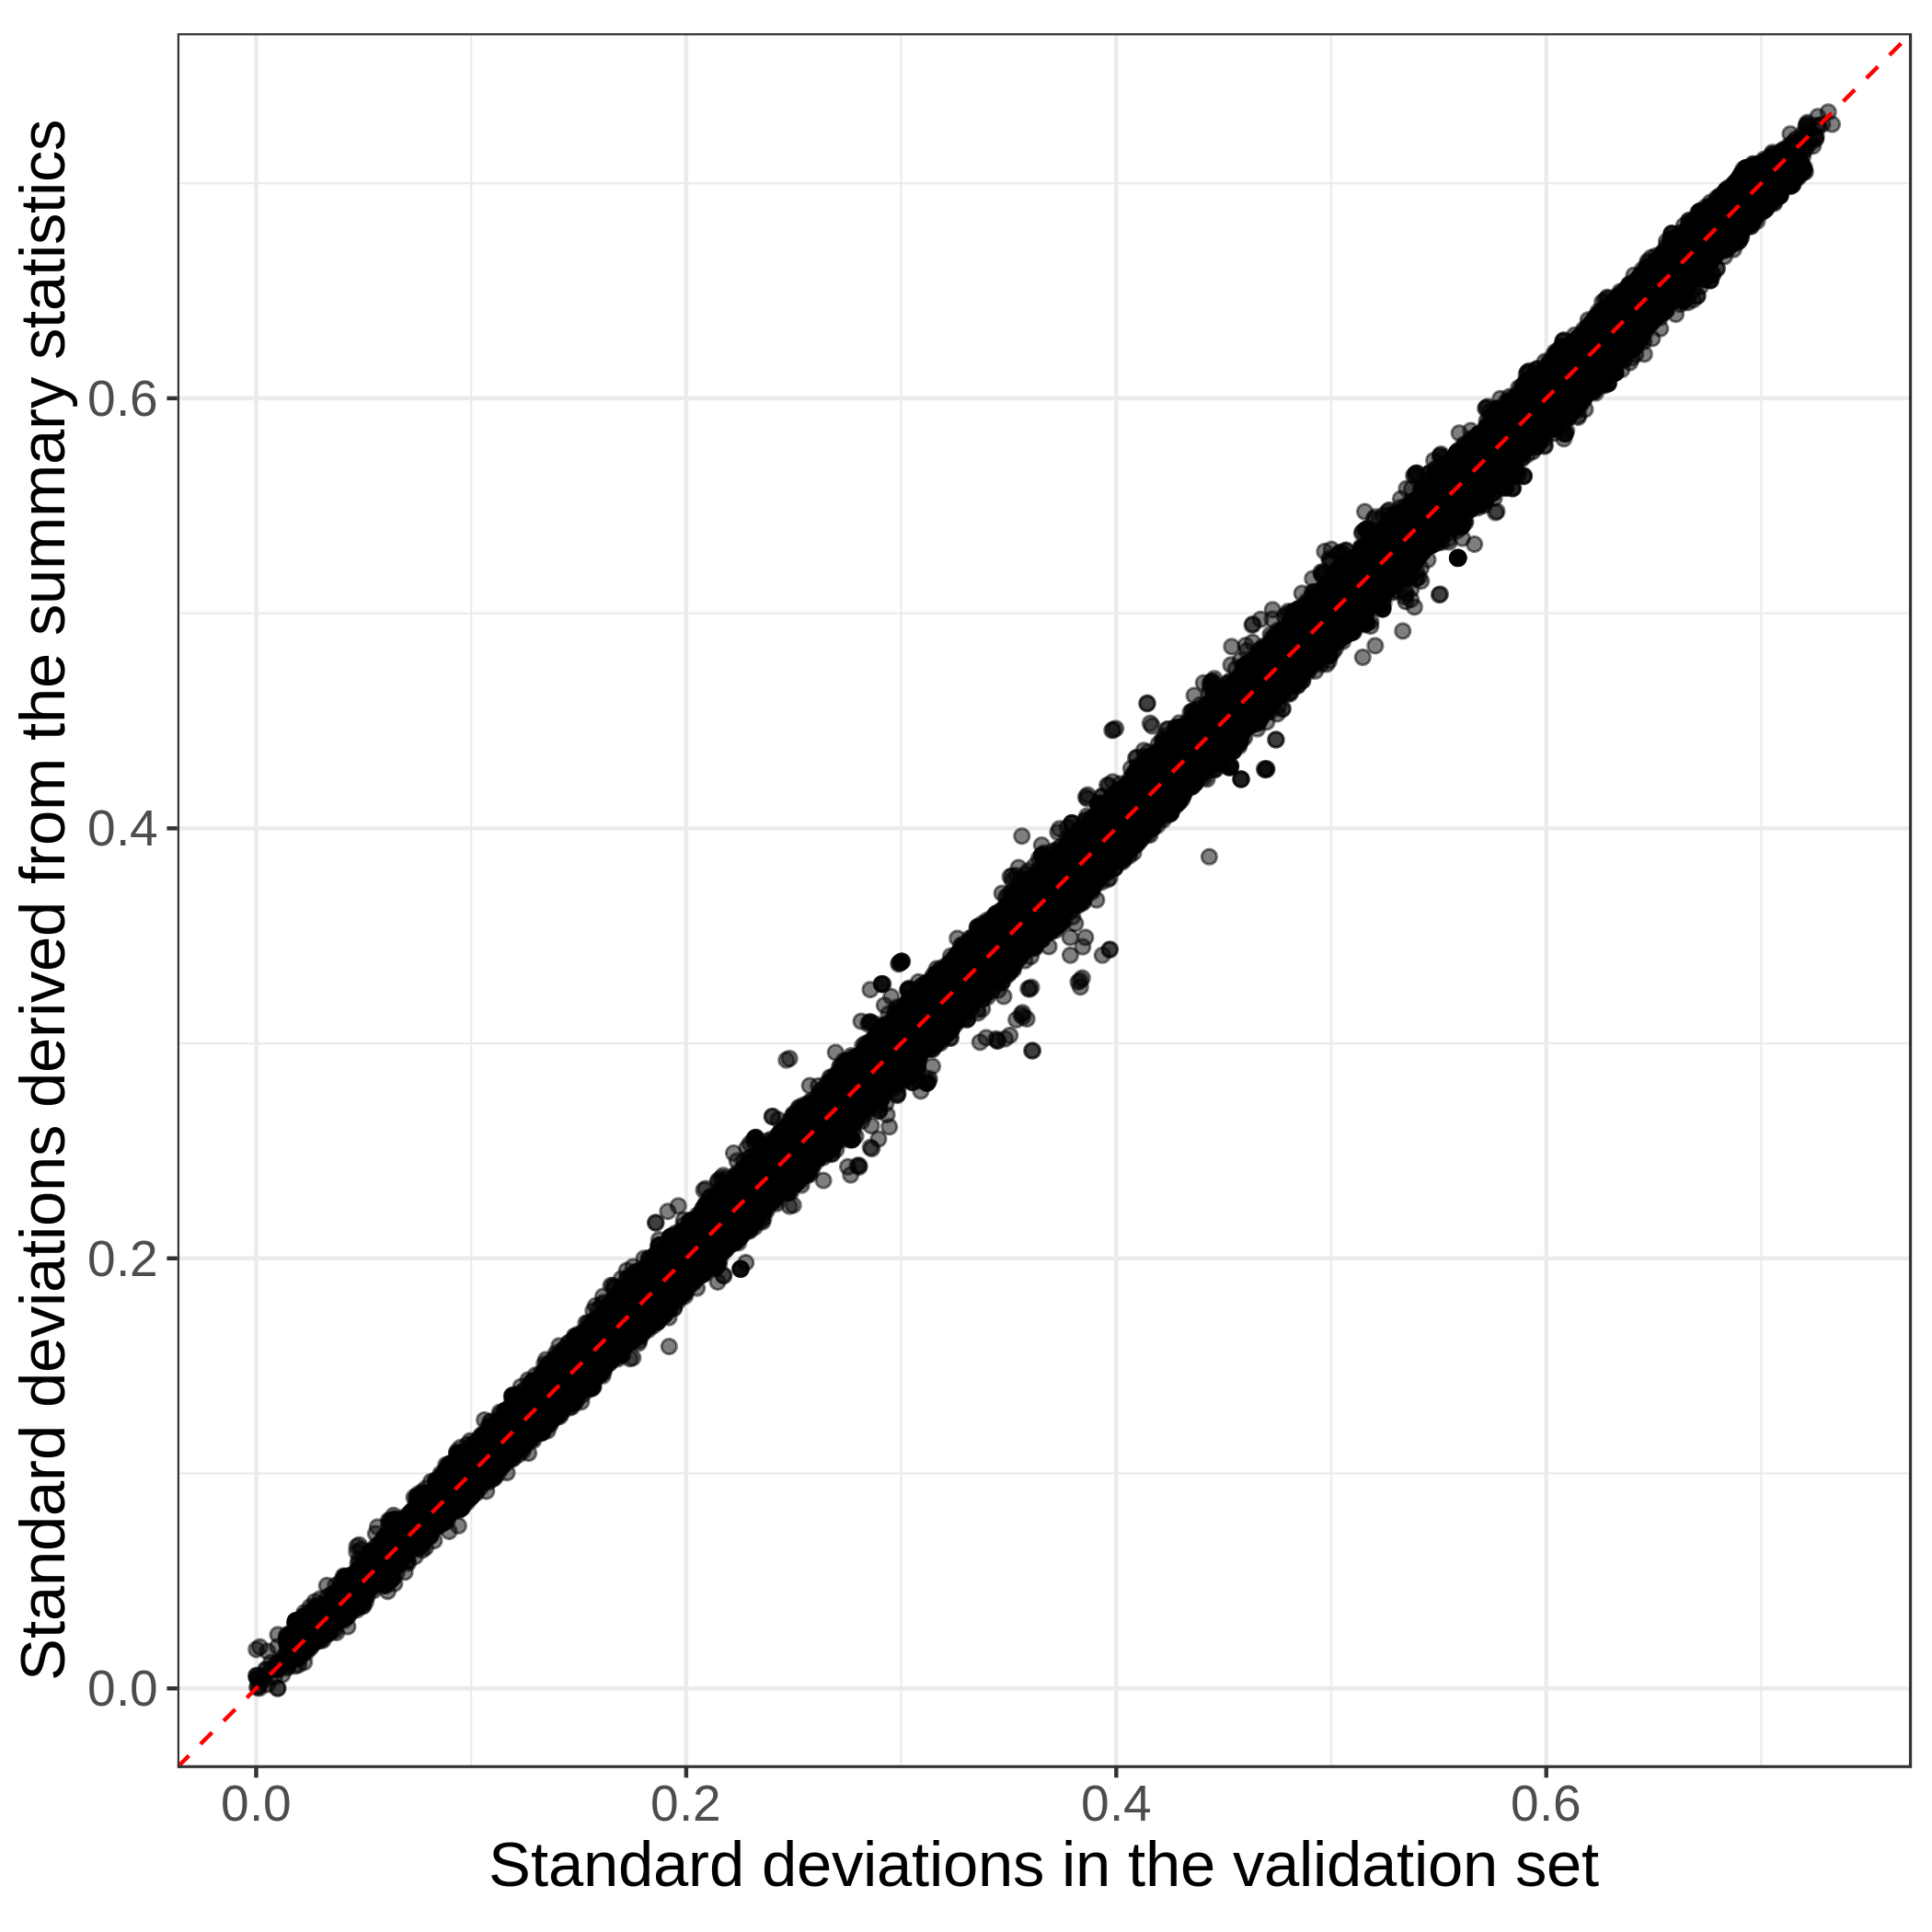
\includegraphics[width=0.7\textwidth]{sd-approx-simu}}
	\caption{In simulations, standard deviations derived from summary statistics based on equation (3) versus the standard deviations of genotypes of individuals in the validation set.}
	\label{fig:sd-approx-simu}
\end{figure}

\begin{figure}[htbp]
	\centerline{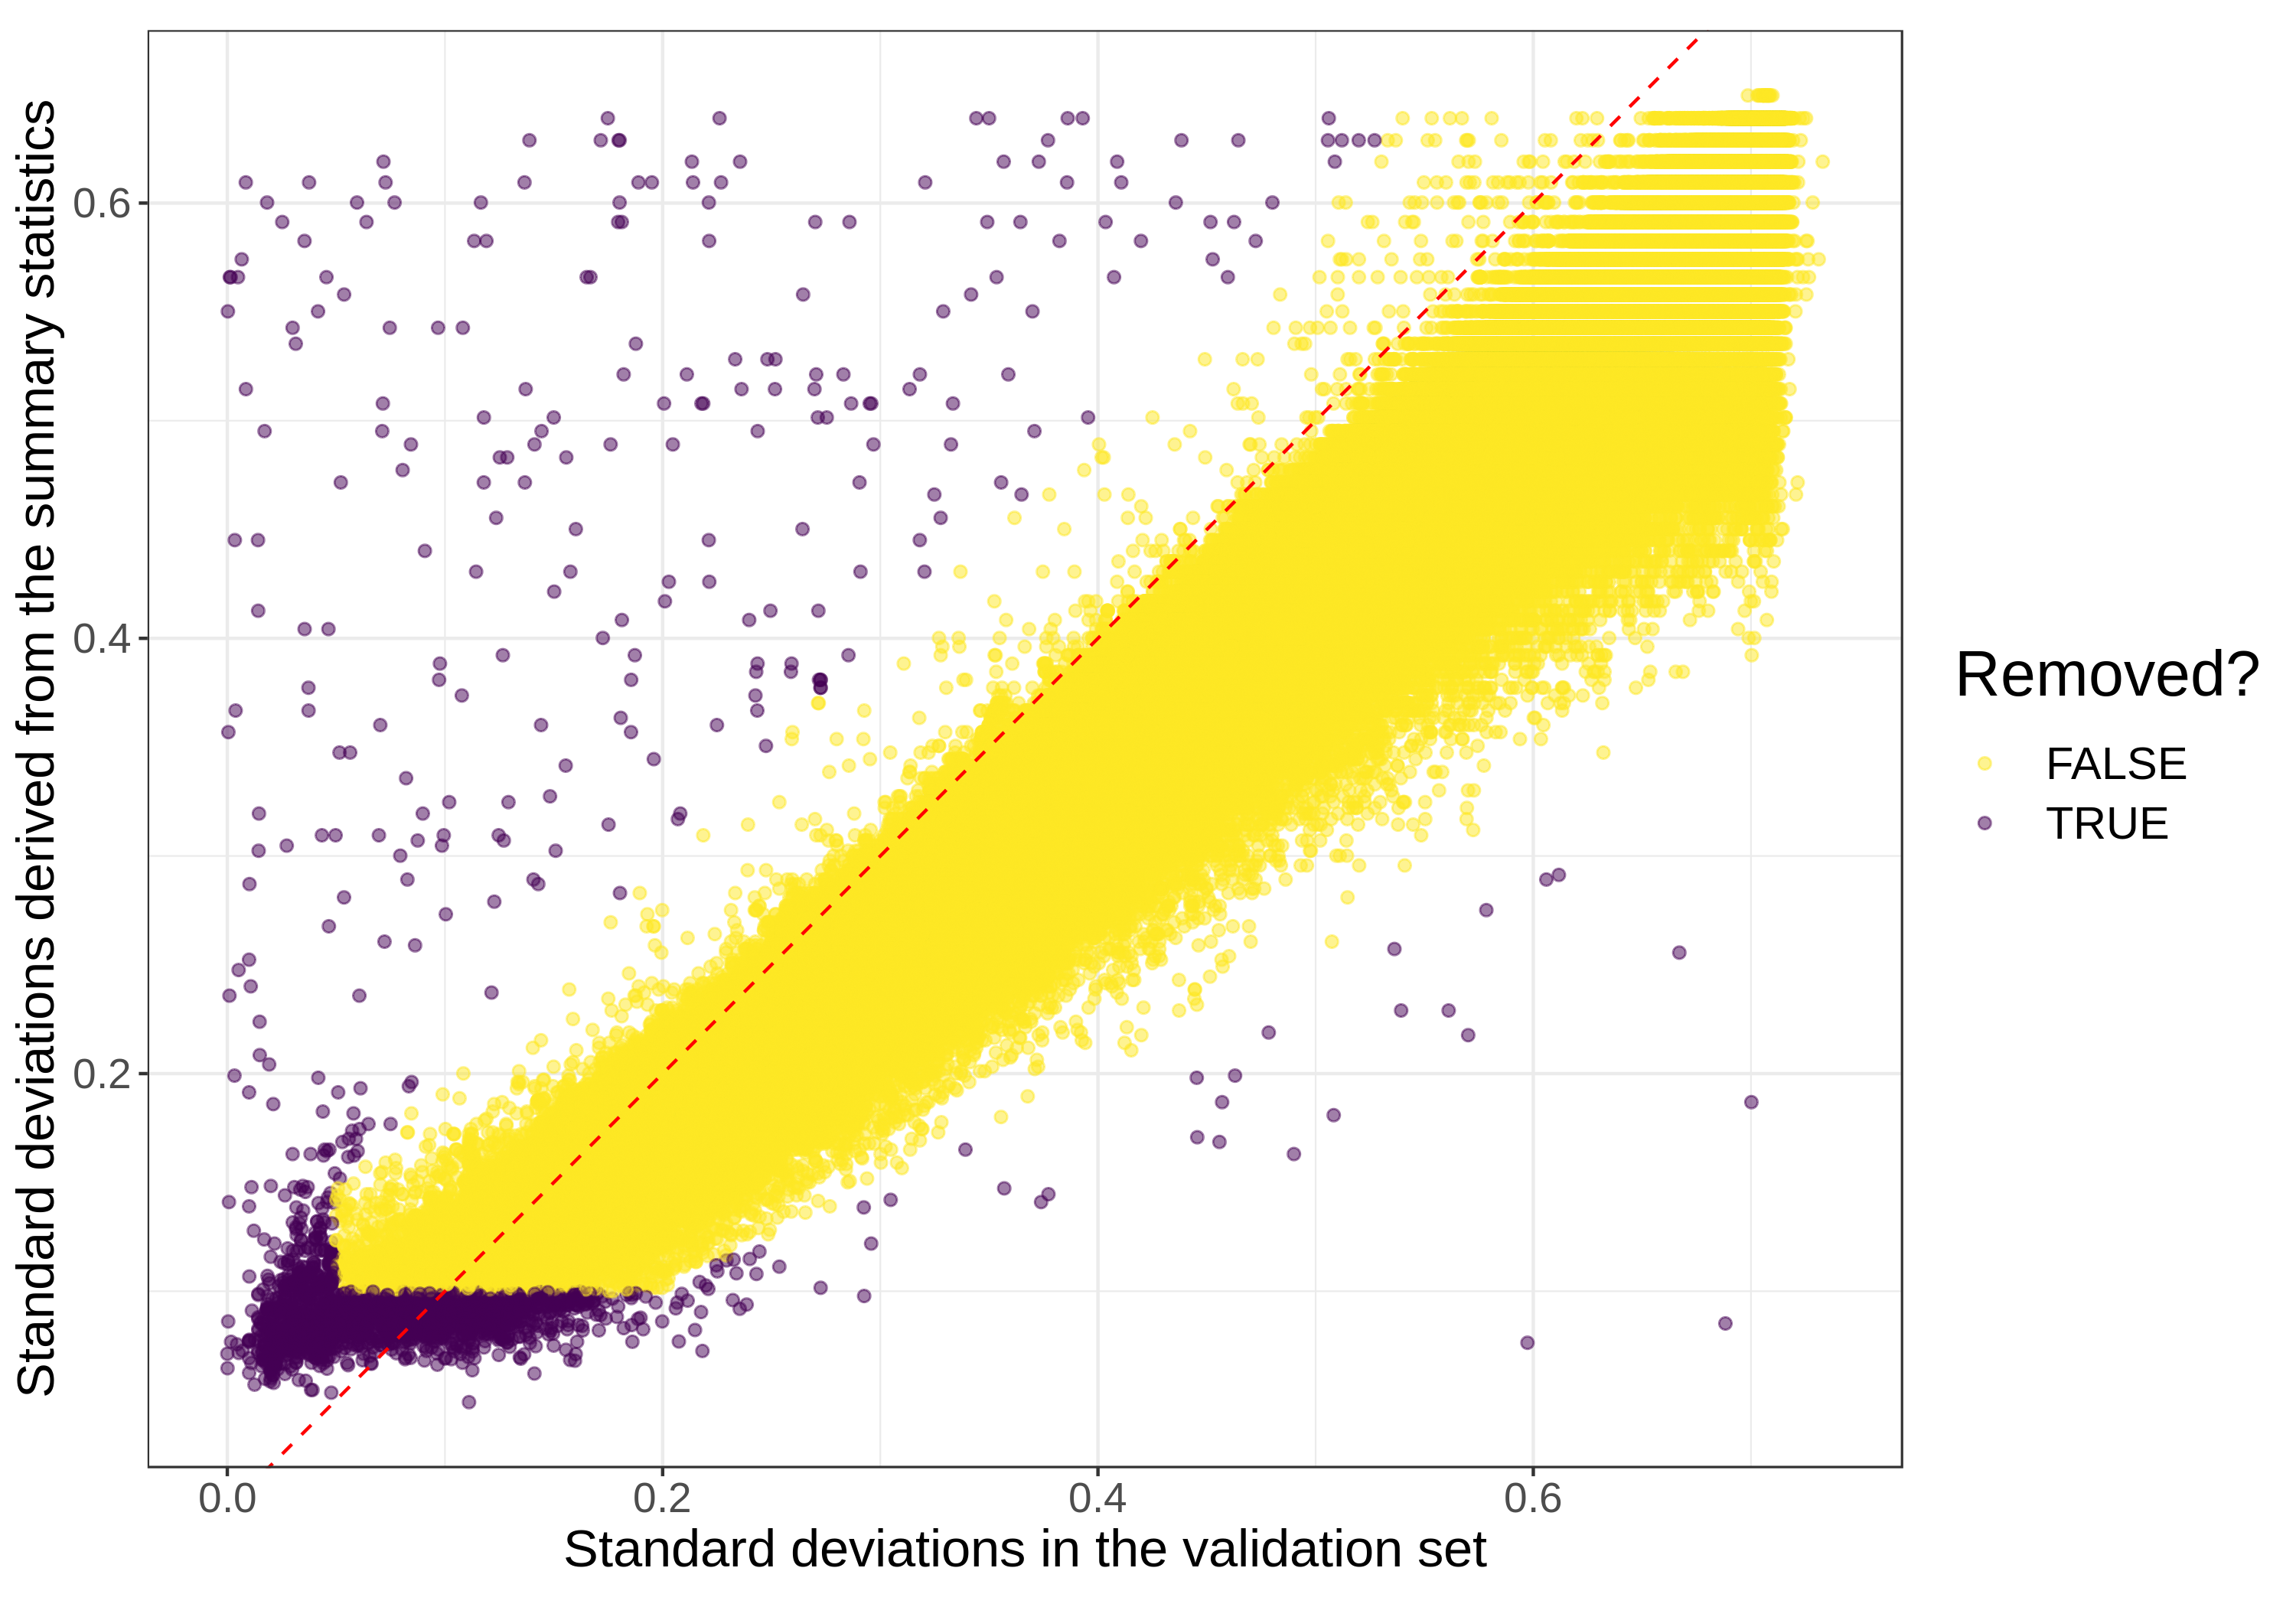
\includegraphics[width=0.9\textwidth]{sd-approx-BRCA}}
	\caption{Standard deviations derived from summary statistics of breast cancer based on equation (3) versus the standard deviations of genotypes of individuals in the validation set. Coloring shows the quality control applied in this paper.}
	\label{fig:sd-approx-brca}
\end{figure}

\FloatBarrier

%%%%%%%%%%%%%%%%%%%%%%%%%%%%%%%%%%%%%%%%%%%%%%%%%%%%%%%%%%%%%%%%%%%%%%%%%%%%%%%%

\begin{figure}[htbp]
	\centerline{\includegraphics[width=0.9\textwidth]{af-outliers}}
	\caption{Allele frequencies for HapMap3 variants in the 1000 Genomes and in UK Biobank. Variants are removed when the difference between these two frequencies is very significant ($p<10^{-5}$). Variants kept are used to provide an LD reference based on the UK Biobank data.}
	\label{fig:af-outliers}
\end{figure}

%%%%%%%%%%%%%%%%%%%%%%%%%%%%%%%%%%%%%%%%%%%%%%%%%%%%%%%%%%%%%%%%%%%%%%%%%%%%%%%%

\end{document}
